In this section the design of the trajectory is presented. Also the motivation behind it, its sensitivity to changing atmospheric properties and the possibility to correct for these changes are explained. The main input with which the trajectory is calculated is the shape of the aeroshell. This shape and the reasoning behind it is presented in Section \ref{sec:AeroDesign}.

\paragraph{Aerocapture}
The first phase of the trajectory is aerocapture, in this phase the objective is to loose enough energy to get in a mars synchronous orbit. The velocity that has to be obtained at the end of aerocapture is $4.53 \left[km \cdot s^{-1}\right]$
***Trajectory so we come in a Mars synchronous orbit***\\
***As high through the atosphere as possible to facilitate themodynamics and structural masses***\\

***Sensitivity to density change +-10\% and possibility to correct for it***\\
\begin{sidewaysfigure}
	\centering
	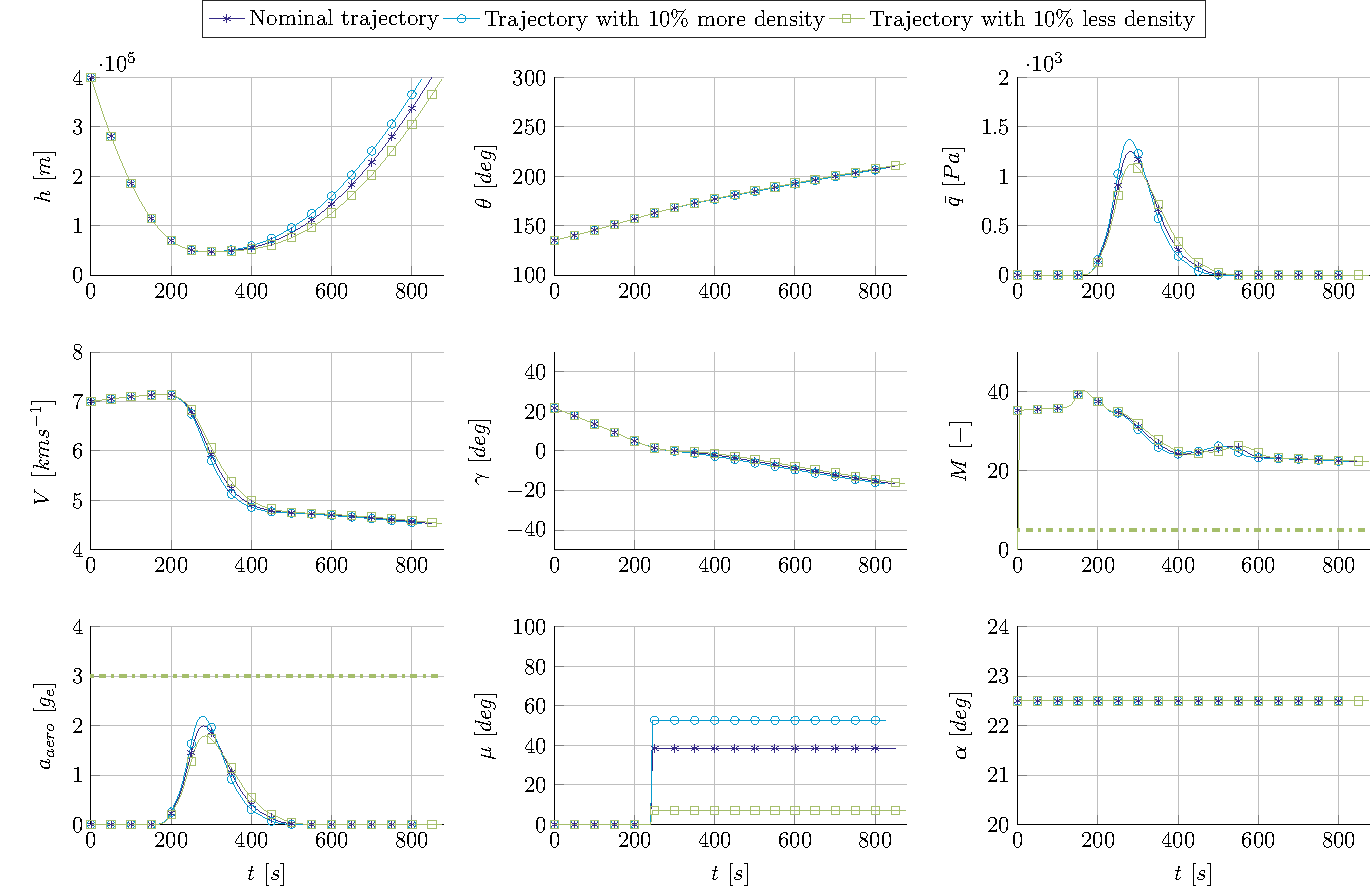
\includegraphics[width=0.99\textwidth]{Figure/Orbit/sensitivity_aerocapture.pdf}
	\caption{ Results of the re-entry trajectory for three different density profiles. The trajectories with modified density are corrected to maintain the same exit velocity. The horizontal dashed lines are design limits (for the \gls{sym:M} and \gls{sym:acc} plots) }
	\label{fig:orbit_aerocapture_data}
\end{sidewaysfigure}

\paragraph{Parking orbit}
***Use of orbit, extrension of time***\\
***Orbital period, 1 sol***\\

\paragraph{Entry and descent}
***Entry conditions imposed by aerocapture and parking orbit***
***trajectory based on 3g requirement \& Mach 5 reuirement***
***$\alpha$ control not nessesary***

***Sensitivity to density change +-10\% and possibility to correct for it***\\
\begin{sidewaysfigure}
	\centering
	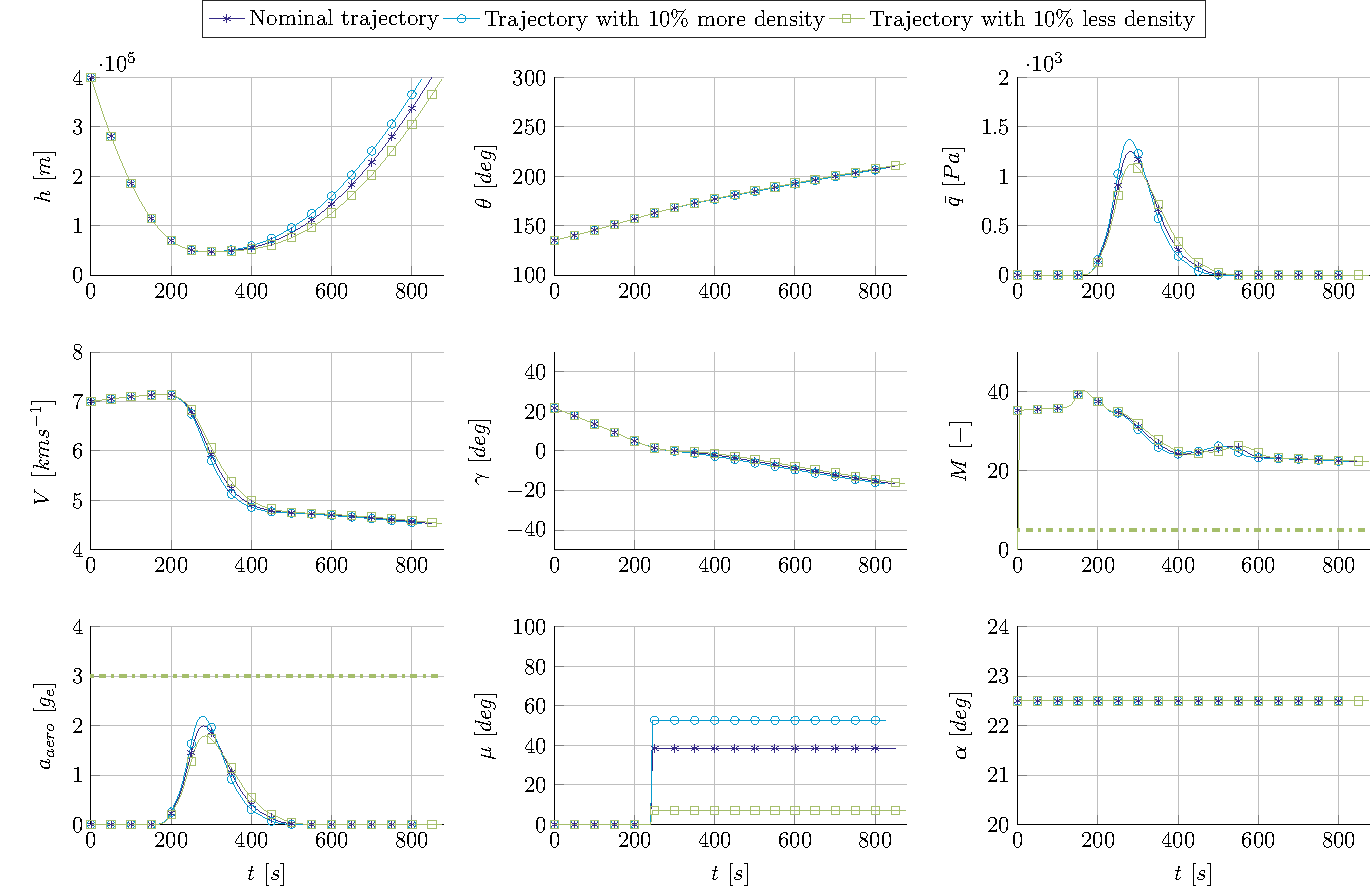
\includegraphics[width=0.99\textwidth]{Figure/Orbit/sensitivity_aerocapture.pdf}
	\caption{Results of the re-entry trajectory for three different density profiles. The trajectories with modified density are corrected to show the ability to reach the desired landing location. The horizontal dashed lines are design limits (for the \gls{sym:M} and \gls{sym:acc} plots)*******************Change this figure***************** }
	\label{fig:orbit_entry_data}
\end{sidewaysfigure}